% Options for packages loaded elsewhere
% Options for packages loaded elsewhere
\PassOptionsToPackage{unicode}{hyperref}
\PassOptionsToPackage{hyphens}{url}
%
\documentclass[
  ignorenonframetext,
  aspectratio=169,
  handout]{beamer}
\newif\ifbibliography
\usepackage{pgfpages}
\setbeamertemplate{caption}[numbered]
\setbeamertemplate{caption label separator}{: }
\setbeamercolor{caption name}{fg=normal text.fg}
\beamertemplatenavigationsymbolsempty
% remove section numbering
\setbeamertemplate{part page}{
  \centering
  \begin{beamercolorbox}[sep=16pt,center]{part title}
    \usebeamerfont{part title}\insertpart\par
  \end{beamercolorbox}
}
\setbeamertemplate{section page}{
  \centering
  \begin{beamercolorbox}[sep=12pt,center]{section title}
    \usebeamerfont{section title}\insertsection\par
  \end{beamercolorbox}
}
\setbeamertemplate{subsection page}{
  \centering
  \begin{beamercolorbox}[sep=8pt,center]{subsection title}
    \usebeamerfont{subsection title}\insertsubsection\par
  \end{beamercolorbox}
}
% Prevent slide breaks in the middle of a paragraph
\widowpenalties 1 10000
\raggedbottom
\AtBeginPart{
  \frame{\partpage}
}
\AtBeginSection{
  \ifbibliography
  \else
    \frame{\sectionpage}
  \fi
}
\AtBeginSubsection{
  \frame{\subsectionpage}
}
\usepackage{iftex}
\ifPDFTeX
  \usepackage[T1]{fontenc}
  \usepackage[utf8]{inputenc}
  \usepackage{textcomp} % provide euro and other symbols
\else % if luatex or xetex
  \usepackage{unicode-math} % this also loads fontspec
  \defaultfontfeatures{Scale=MatchLowercase}
  \defaultfontfeatures[\rmfamily]{Ligatures=TeX,Scale=1}
\fi
\usepackage{lmodern}

\ifPDFTeX\else
  % xetex/luatex font selection
\fi
% Use upquote if available, for straight quotes in verbatim environments
\IfFileExists{upquote.sty}{\usepackage{upquote}}{}
\IfFileExists{microtype.sty}{% use microtype if available
  \usepackage[]{microtype}
  \UseMicrotypeSet[protrusion]{basicmath} % disable protrusion for tt fonts
}{}
\makeatletter
\@ifundefined{KOMAClassName}{% if non-KOMA class
  \IfFileExists{parskip.sty}{%
    \usepackage{parskip}
  }{% else
    \setlength{\parindent}{0pt}
    \setlength{\parskip}{6pt plus 2pt minus 1pt}}
}{% if KOMA class
  \KOMAoptions{parskip=half}}
\makeatother


\usepackage{longtable,booktabs,array}
\newcounter{none} % for unnumbered tables
\usepackage{calc} % for calculating minipage widths
\usepackage{caption}
% Make caption package work with longtable
\makeatletter
\def\fnum@table{\tablename~\thetable}
\makeatother
\usepackage{graphicx}
\makeatletter
\newsavebox\pandoc@box
\newcommand*\pandocbounded[1]{% scales image to fit in text height/width
  \sbox\pandoc@box{#1}%
  \Gscale@div\@tempa{\textheight}{\dimexpr\ht\pandoc@box+\dp\pandoc@box\relax}%
  \Gscale@div\@tempb{\linewidth}{\wd\pandoc@box}%
  \ifdim\@tempb\p@<\@tempa\p@\let\@tempa\@tempb\fi% select the smaller of both
  \ifdim\@tempa\p@<\p@\scalebox{\@tempa}{\usebox\pandoc@box}%
  \else\usebox{\pandoc@box}%
  \fi%
}
% Set default figure placement to htbp
\def\fps@figure{htbp}
\makeatother





\setlength{\emergencystretch}{3em} % prevent overfull lines

\providecommand{\tightlist}{%
  \setlength{\itemsep}{0pt}\setlength{\parskip}{0pt}}



 


\makeatletter
\@ifpackageloaded{caption}{}{\usepackage{caption}}
\AtBeginDocument{%
\ifdefined\contentsname
  \renewcommand*\contentsname{Table of contents}
\else
  \newcommand\contentsname{Table of contents}
\fi
\ifdefined\listfigurename
  \renewcommand*\listfigurename{List of Figures}
\else
  \newcommand\listfigurename{List of Figures}
\fi
\ifdefined\listtablename
  \renewcommand*\listtablename{List of Tables}
\else
  \newcommand\listtablename{List of Tables}
\fi
\ifdefined\figurename
  \renewcommand*\figurename{Figure}
\else
  \newcommand\figurename{Figure}
\fi
\ifdefined\tablename
  \renewcommand*\tablename{Table}
\else
  \newcommand\tablename{Table}
\fi
}
\@ifpackageloaded{float}{}{\usepackage{float}}
\floatstyle{ruled}
\@ifundefined{c@chapter}{\newfloat{codelisting}{h}{lop}}{\newfloat{codelisting}{h}{lop}[chapter]}
\floatname{codelisting}{Listing}
\newcommand*\listoflistings{\listof{codelisting}{List of Listings}}
\makeatother
\makeatletter
\makeatother
\makeatletter
\@ifpackageloaded{caption}{}{\usepackage{caption}}
\@ifpackageloaded{subcaption}{}{\usepackage{subcaption}}
\makeatother

\usepackage{bookmark}
\IfFileExists{xurl.sty}{\usepackage{xurl}}{} % add URL line breaks if available
\urlstyle{same}
\hypersetup{
  pdftitle={The Rigid Rotor},
  pdfauthor={Davit Potoyan},
  hidelinks,
  pdfcreator={LaTeX via pandoc}}


\title{\texorpdfstring{The Rigid Rotor}{The Rigid Rotor}}
\subtitle{\texorpdfstring{Chem 3240 · Lecture
4.6}{Chem 3240 · Lecture 4.6}}
\author{Davit Potoyan}
\date{}

\begin{document}
\frame{\titlepage}


\begin{frame}
\begin{block}{The model}
\protect\phantomsection\label{the-model}
\begin{columns}[T]
\begin{column}{0.55\linewidth}
\begin{itemize}
\tightlist
\item
  A mass \(\mu\) rotating at \textbf{fixed radius} \(r\)
\end{itemize}

\begin{itemize}
\tightlist
\item
  No potential: pure rotational \textbf{kinetic energy}
\end{itemize}

\begin{itemize}
\tightlist
\item
  Use \textbf{spherical coordinates} to exploit the symmetry
\end{itemize}

\begin{itemize}
\tightlist
\item
  Hamiltonian becomes angular momentum: \[\hat{H}=\frac{\hat{L}^2}{2I}\]
\end{itemize}
\end{column}

\begin{column}{0.45\linewidth}
\pandocbounded{\includegraphics[keepaspectratio]{../../ch04/images/sphhar.gif}}
\end{column}
\end{columns}
\end{block}

\begin{block}{Two angles, two quantum numbers}
\protect\phantomsection\label{two-angles-two-quantum-numbers}
Eigenfunctions are the \textbf{spherical harmonics} \(Y(\theta,\phi)\):
\[\hat{H}\,Y(\theta,\phi)=E_{J,m}\,Y(\theta,\phi)\]

\begin{itemize}
\tightlist
\item
  \(J\) quantizes total angular momentum
\end{itemize}

\begin{itemize}
\tightlist
\item
  \(M_J\) quantizes its projection
\end{itemize}

\begin{itemize}
\tightlist
\item
  Quantization comes from the \textbf{cyclic boundary condition}
  \(\Phi(0)=\Phi(2\pi)\)
\end{itemize}
\end{block}

\begin{block}{Rotational energy levels}
\protect\phantomsection\label{rotational-energy-levels}
\[E_J = \frac{\hbar^2}{2I}J(J+1) = B\,J(J+1)\]

\textbf{Rotational constant} (units of energy):
\[B = \frac{h^2}{8\pi^2 I}\]

\begin{itemize}
\tightlist
\item
  Energy depends \textbf{only on \(J\)}
\end{itemize}

\begin{itemize}
\tightlist
\item
  \textbf{No zero-point energy}: \(J=0\) is allowed
\end{itemize}
\end{block}

\begin{block}{Degeneracy and the moment of inertia}
\protect\phantomsection\label{degeneracy-and-the-moment-of-inertia}
\begin{columns}[T]
\begin{column}{0.5\linewidth}
Each level is \textbf{\((2J+1)\)-fold degenerate} (the allowed \(M_J\))

For a diatomic: \[I = \mu r^2\]

\begin{itemize}
\tightlist
\item
  Bigger \(I\) \(\Rightarrow\) smaller \(B\) \(\Rightarrow\) closer
  levels
\end{itemize}
\end{column}

\begin{column}{0.5\linewidth}
\pandocbounded{\includegraphics[keepaspectratio]{../../ch04/images/Levels1.gif}}
\end{column}
\end{columns}
\end{block}

\begin{block}{Selection rules}
\protect\phantomsection\label{selection-rules}
The molecule must have a \textbf{permanent dipole moment}:
\[\langle J' | \mu | J'' \rangle \neq 0\]

Only adjacent levels connect: \[\boxed{\Delta J = \pm 1}\]

\begin{itemize}
\tightlist
\item
  Derived from the \textbf{recursion relations} of spherical harmonics
\end{itemize}
\end{block}

\begin{block}{Evenly spaced lines}
\protect\phantomsection\label{evenly-spaced-lines}
Line positions (\(\Delta J = +1\)): \[\tilde{\nu}_J = 2\tilde{B}(J+1)\]

Take one more difference:
\[\tilde{\nu}_{J+1} - \tilde{\nu}_J = 2\tilde{B}\]

\begin{itemize}
\tightlist
\item
  Successive lines at \(2\tilde{B},\,4\tilde{B},\,6\tilde{B},\dots\)
\end{itemize}

\begin{itemize}
\tightlist
\item
  \textbf{Equal spacing} is the fingerprint of the rigid rotor
\end{itemize}
\end{block}

\begin{block}{Reading the spacing}
\protect\phantomsection\label{reading-the-spacing}
\begin{columns}[T]
\begin{column}{0.55\linewidth}
\begin{itemize}
\tightlist
\item
  Measure line spacing \(\Rightarrow\) get \(\tilde{B}\)
\end{itemize}

\begin{itemize}
\tightlist
\item
  \(\tilde{B}\Rightarrow I\Rightarrow\) \textbf{bond length} \(r\)
\end{itemize}

\begin{itemize}
\tightlist
\item
  Different \textbf{isotopes} shift the lines
\end{itemize}

\begin{itemize}
\tightlist
\item
  Intensities follow the \textbf{Boltzmann} populations
  \(g_J\,e^{-E_J/k_BT}\)
\end{itemize}
\end{column}

\begin{column}{0.45\linewidth}
\pandocbounded{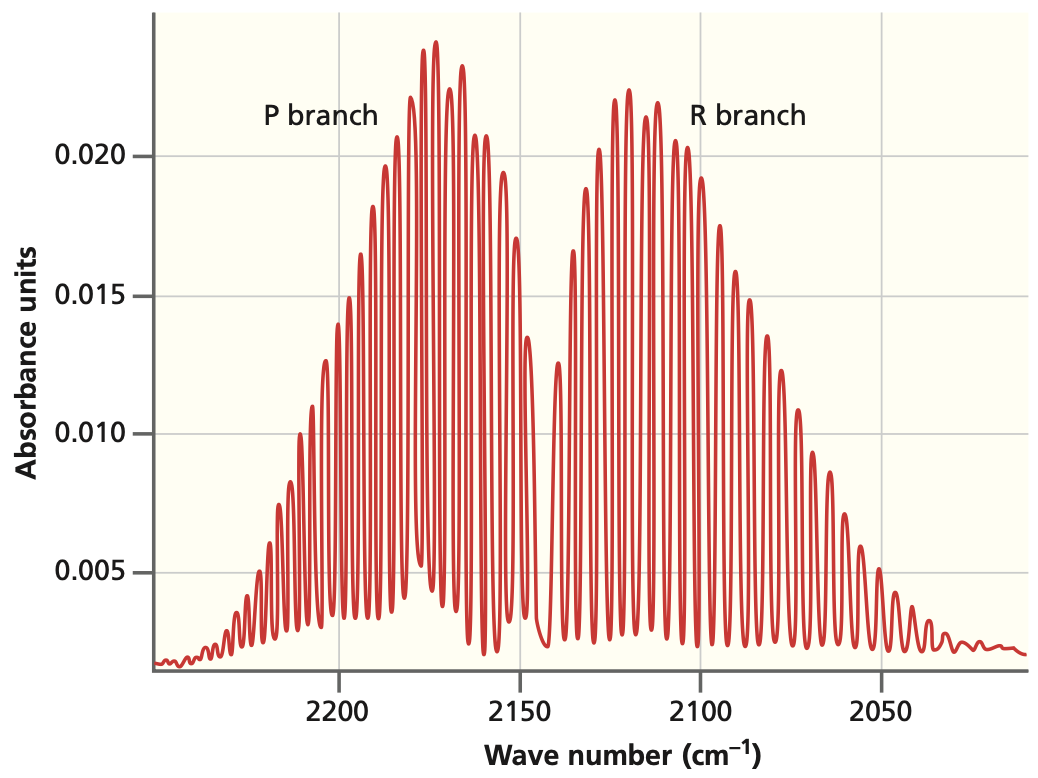
\includegraphics[keepaspectratio]{../../ch04/images/co_micr.png}}
\end{column}
\end{columns}
\end{block}

\begin{block}{Rotation rides on vibration}
\protect\phantomsection\label{rotation-rides-on-vibration}
\begin{columns}[T]
\begin{column}{0.5\linewidth}
Combine rotor and oscillator:
\[\tilde{E}_{v,J} = \tilde{\omega}(v+\tfrac12) + \tilde{B}J(J+1)\]

\begin{itemize}
\tightlist
\item
  \textbf{R branch} (\(\Delta J=+1\)): high side of \(\tilde{\omega}\)
\end{itemize}

\begin{itemize}
\tightlist
\item
  \textbf{P branch} (\(\Delta J=-1\)): low side
\end{itemize}

\begin{itemize}
\tightlist
\item
  \textbf{Q branch} (\(\Delta J=0\)) is \textbf{forbidden}
\end{itemize}
\end{column}

\begin{column}{0.5\linewidth}
\pandocbounded{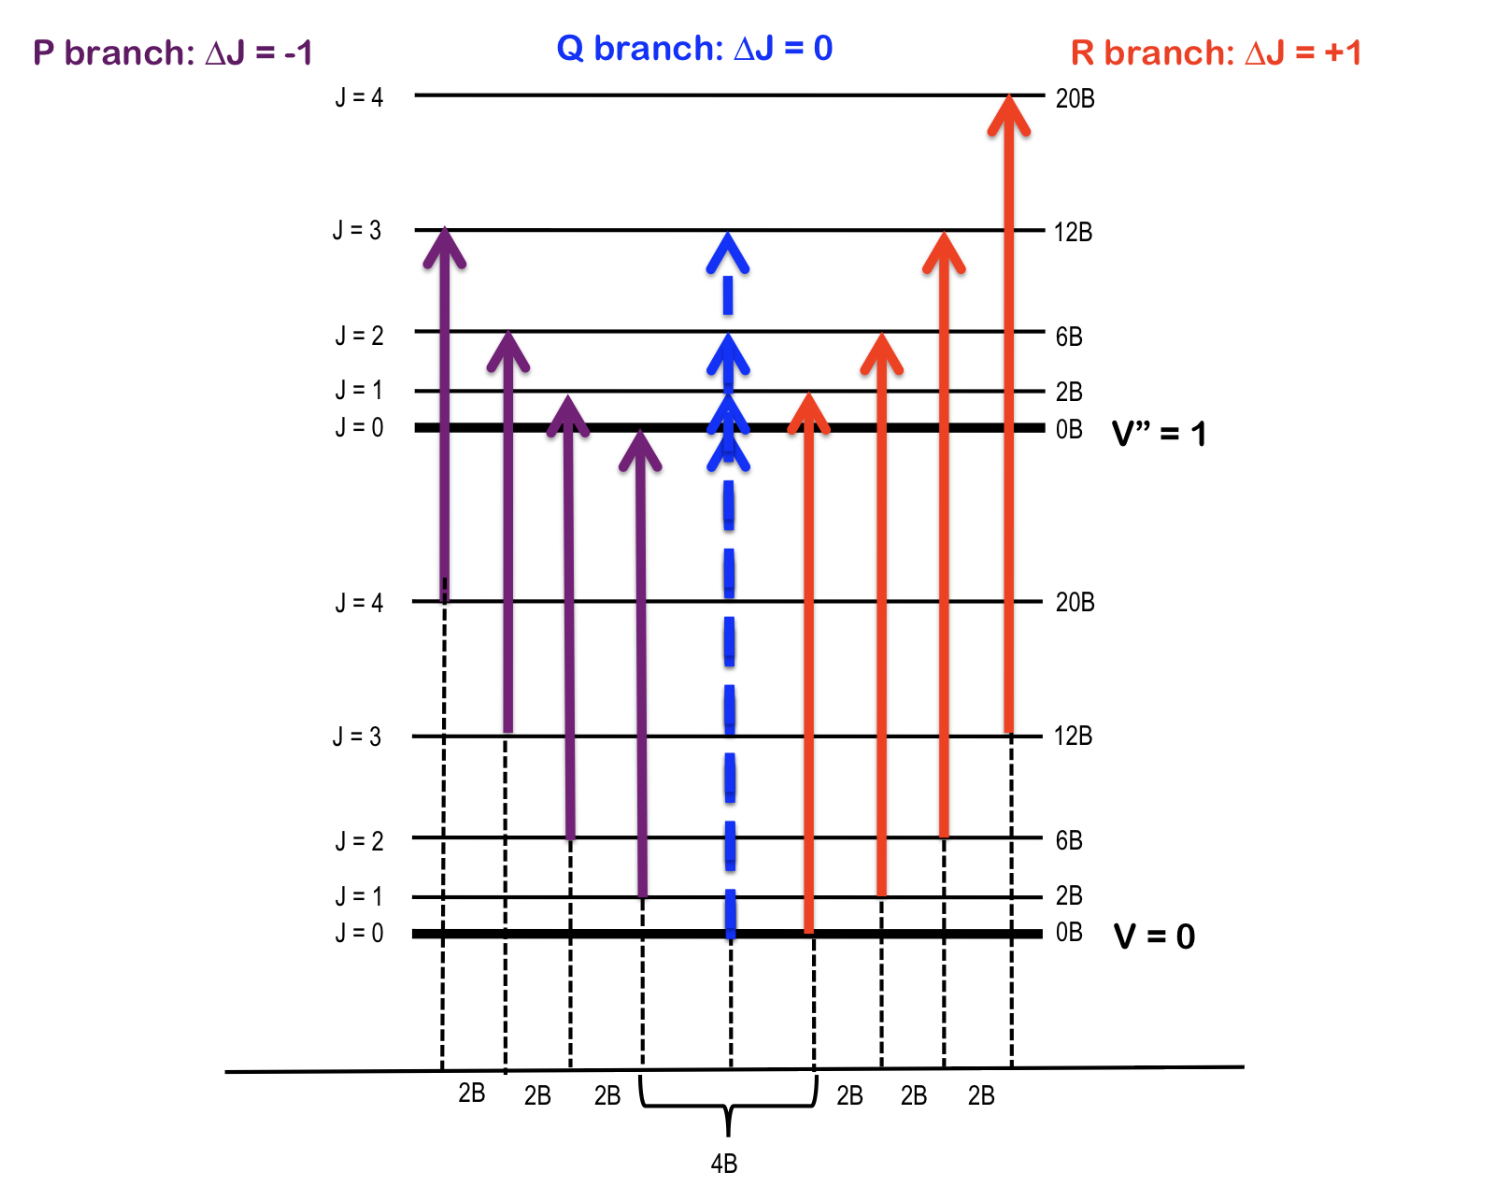
\includegraphics[keepaspectratio]{../../ch04/images/P_Q_R_branch.png}}
\end{column}
\end{columns}
\end{block}

\begin{block}{Where the model breaks}
\protect\phantomsection\label{where-the-model-breaks}
\begin{itemize}
\tightlist
\item
  \textbf{Rovibrational coupling}: \(B\) shrinks with \(v\)
  \[B_v = B_e - \alpha_e(v+\tfrac12)\]
\end{itemize}

\begin{itemize}
\tightlist
\item
  \textbf{Centrifugal distortion}: fast rotation stretches the bond
  \[\tilde{E}_r(J) = \tilde{B}J(J+1) - \tilde{D}J^2(J+1)^2\]
\end{itemize}

\begin{itemize}
\tightlist
\item
  Both crowd the levels at large \(J\)
\end{itemize}
\end{block}
\end{frame}

\begin{frame}{Takeaway}
\protect\phantomsection\label{takeaway}
\begin{quote}
Rotational energies \(E_J = B\,J(J+1)\) are \((2J+1)\)-fold degenerate.
With \(\Delta J=\pm 1\) this gives \textbf{evenly spaced microwave
lines} separated by \(2\tilde{B}\), and the spacing reveals the bond
length through \(I=\mu r^2\).
\end{quote}
\end{frame}




\end{document}
